
% Created 2021-10-29 Fri 15:30

% Intended LaTeX compiler: pdflatex
\documentclass[bigger]{beamer}
\usepackage{graphbox,graphics,graphicx,rotating,xcolor,pgf,tikz,pgfplots}
\usepackage{xspace}
\def\tdsapp{3D Scanner App\xspace}
\mode<beamer>{\usetheme{Madrid}}
\def\lb#1{../../../../../../../home/dek8v5/Dropbox/graphos_reprints/references/bibliography/#1.bib}
\def\tlb#1{../../../../../../Dropbox/graphos_reprints/references/bibliography/#1.bib}
\def\gb#1{../../../../zu_lesen/references/bibliography/#1.bib}
\def\bp{\lb}
\usetheme{default}

\author{Dewi Endah Kharismawati, Chimdi Walter Ndubuisi, and Toni Kazic}
\date{\textit{29 Oct 2021}}
\title{3D plant morphology in the field: experiments with a consumer LiDAR device}

\title[3D Field Plants with LiDAR]{3D plant morphology in the field: experiments with a consumer LiDAR device}
\author[Kharismawati \emph{et al.}]{Dewi Endah Kharismawati, Chimdi Walter Ndubuisi, and Toni Kazic}
\institute{University of Missouri}
\begin{document}


\maketitle
\section{90" talk outline}
\label{sec:org280a454}







\begin{frame}[label={sec:org42af857}]{Rationale}
\begin{itemize}
\item 3D reconstructions often use Structure from Motions (SfM) of 360\(^o\)
RGB videos, but can benefit from depth information.
\item LiDAR is less sensitive to ambient light, making it a
very good candidate for agricultural applications.
\item LiDAR is now available in consumer grade devices, such as
Apple's iPads and iPhones.
\item There are many free applications to get 3D point clouds.
\item We explored 2 apps for collecting point clouds of field plants:
\tdsapp and Scaniverse.
\end{itemize}
\end{frame}


\begin{frame}[label={sec:orgcbc1cd7}]{Point Cloud Quality depends on Plant Morphology}

\centering

% this is ../b/artistry/papers/current/mlcas2021_poster/images/lidar_tableau.tex
%
% this is the transposed figure we used in the extended abstract
%
% Kazic, 27.10.2021



% fixed vertical alignment with graphbox per
% https://tex.stackexchange.com/questions/19080/how-to-vertically-center-text-with-an-image-in-the-same-row-of-a-table
%
% Kazic, 2.10.2021



%
\scalebox{0.75}{%
\begin{tabular}{cccc}
%
% this is the transpose: plants as rows and outputs as columns
%
% rgb
%
& & \multicolumn{2}{c}{raw point clouds} \\
& \textsc{RGB} & \tdsapp & Scaniverse \\
%
\emph{soybean} &
\scalebox{0.08}{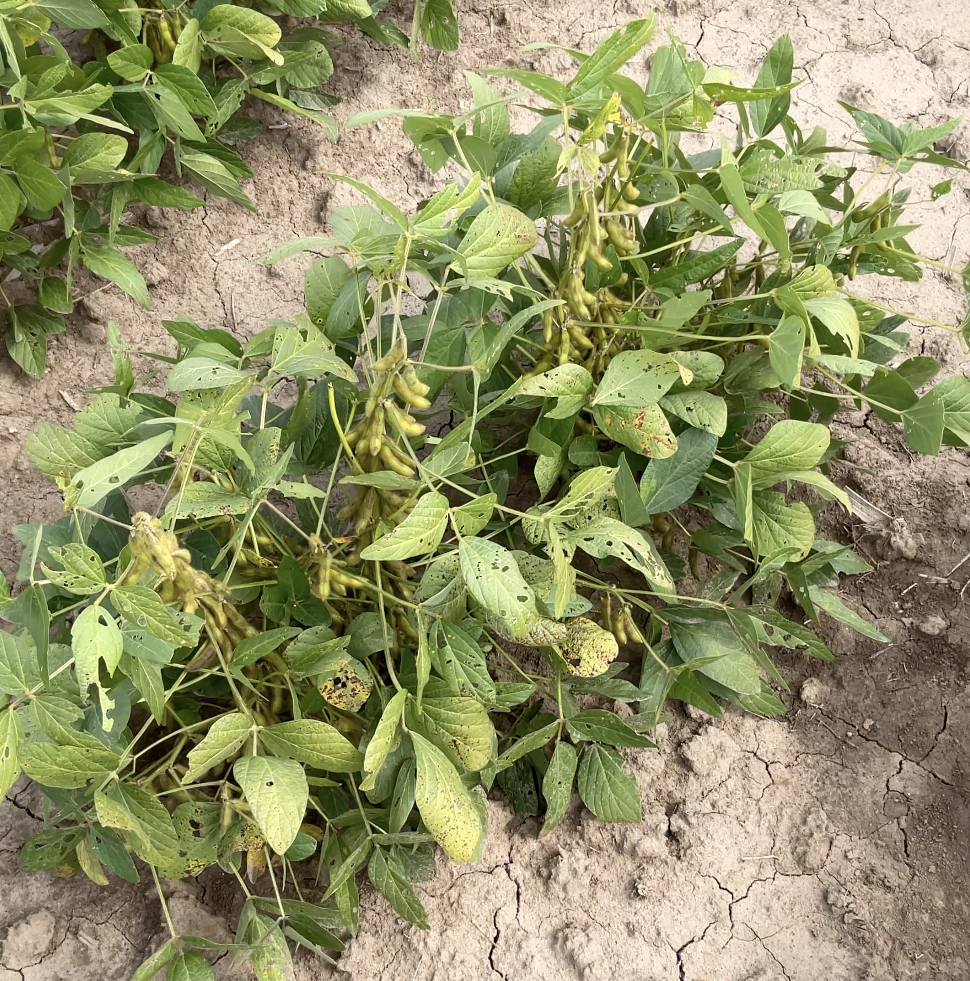
\includegraphics[align=c]{./images/meshlab/soybean3_rgb.png}} &
\scalebox{0.10}{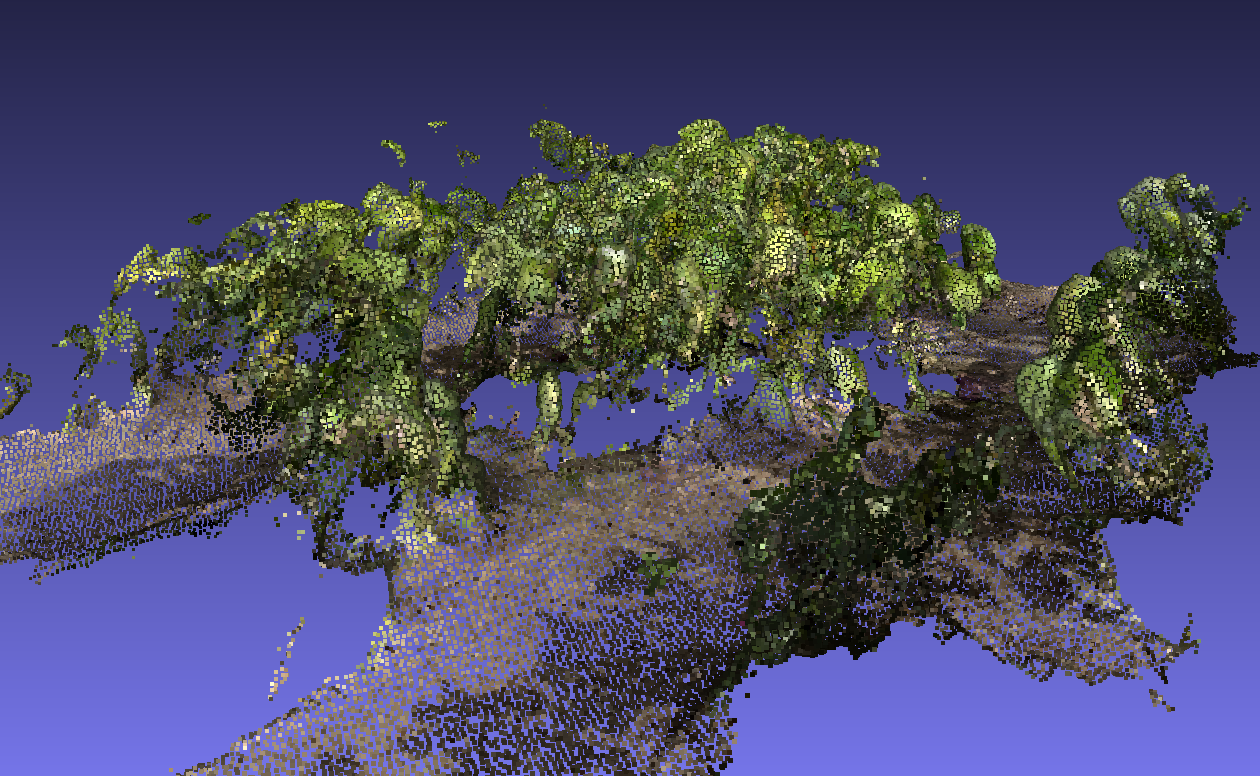
\includegraphics[align=c]{./images/meshlab/soybean3_3dscanner_pc.png}} &
\scalebox{0.10}{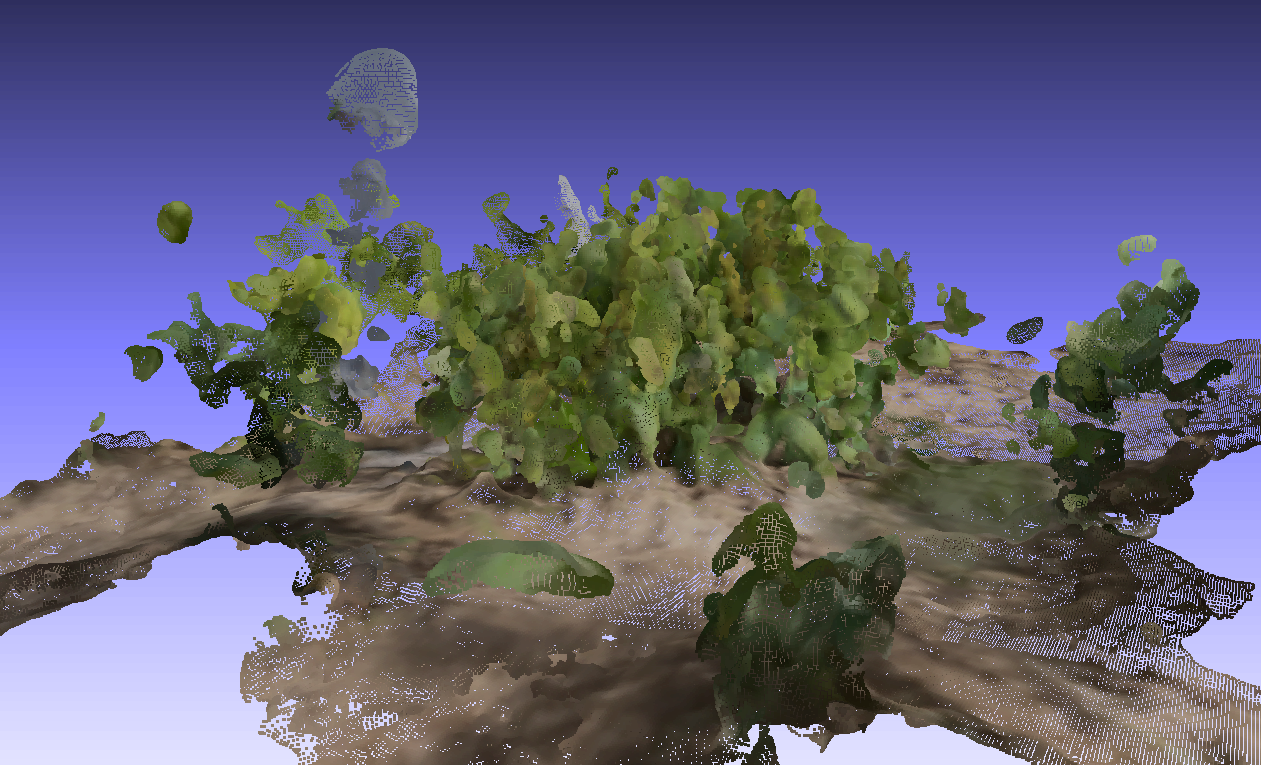
\includegraphics[align=c]{./images/meshlab/soybean3_scaniverse_pc.png}}  \\
%
\emph{cocklebur} &
\scalebox{0.175}{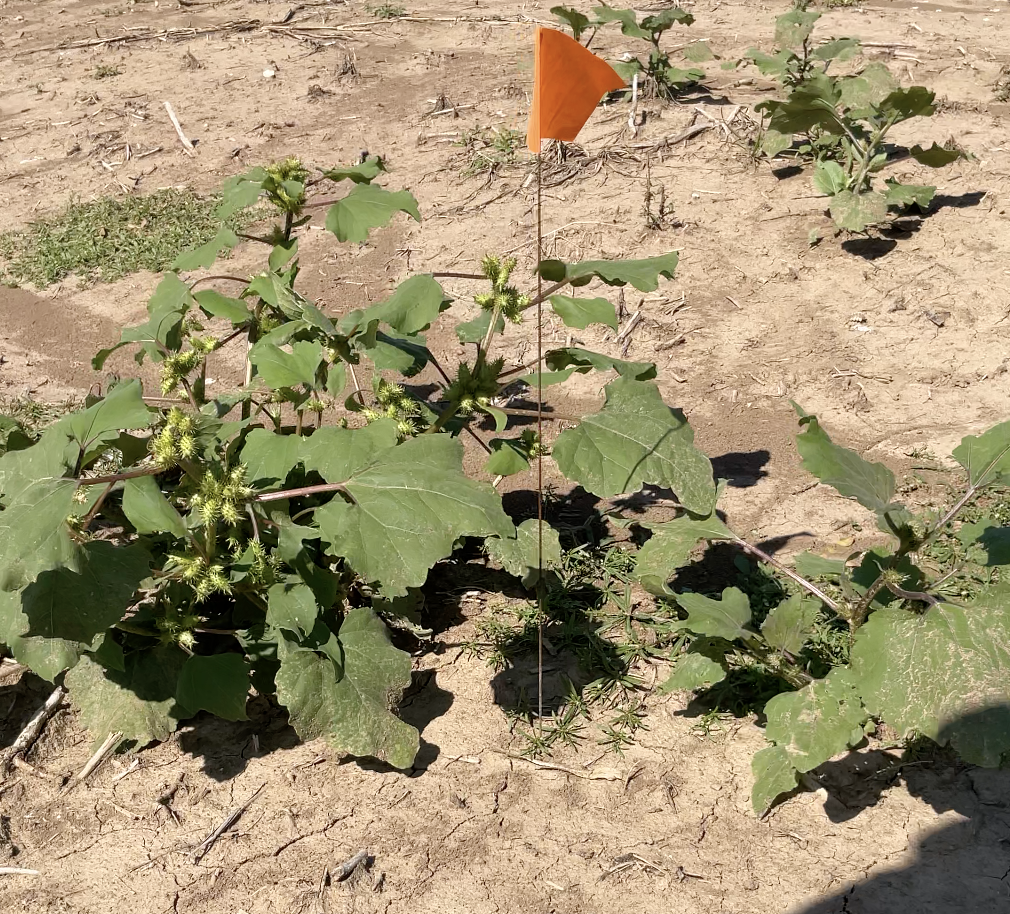
\includegraphics[align=c]{./images/meshlab/cocklebur2_rgb.png}} &
\scalebox{0.11}{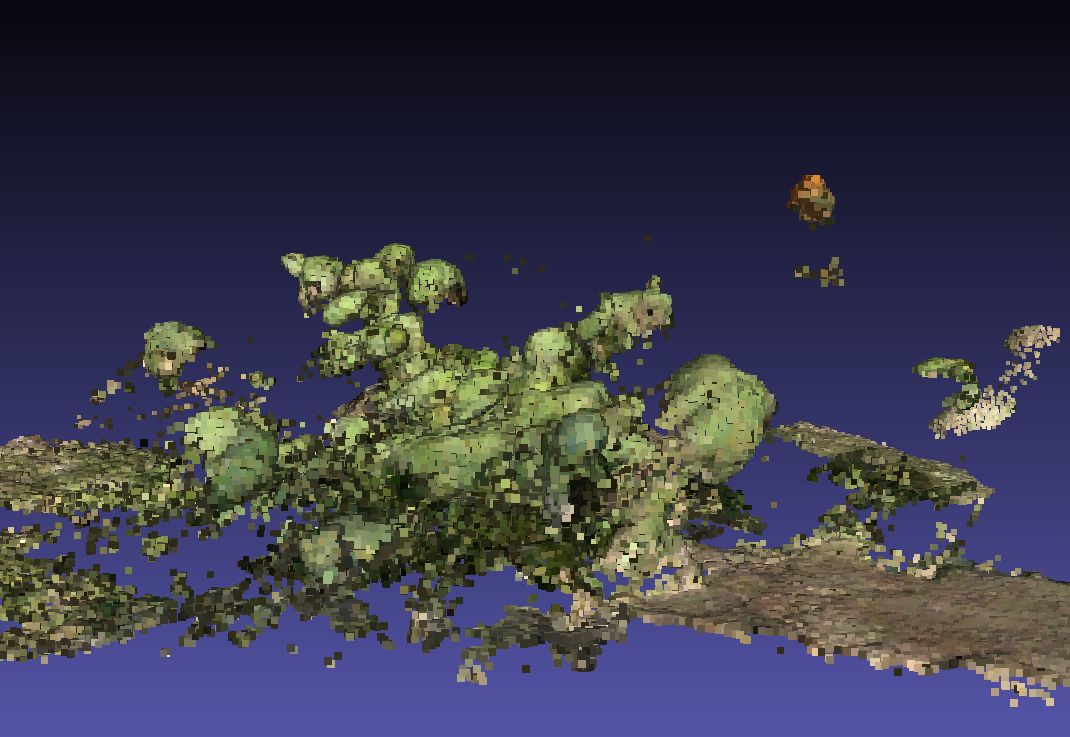
\includegraphics[align=c]{./images/meshlab/cocklebur2_3dscanner_pc.png}} &
\scalebox{0.115}{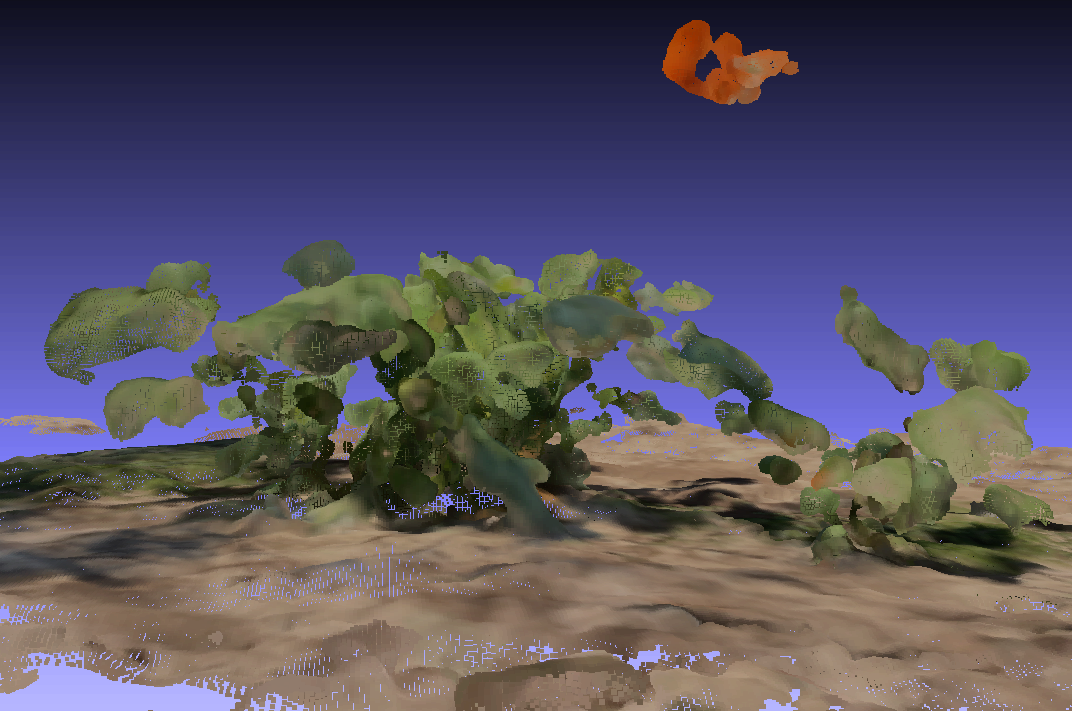
\includegraphics[align=c]{./images/meshlab/cocklebur2_scaniverse_pc.png}} \\
%
\emph{maize} &
\scalebox{0.14}{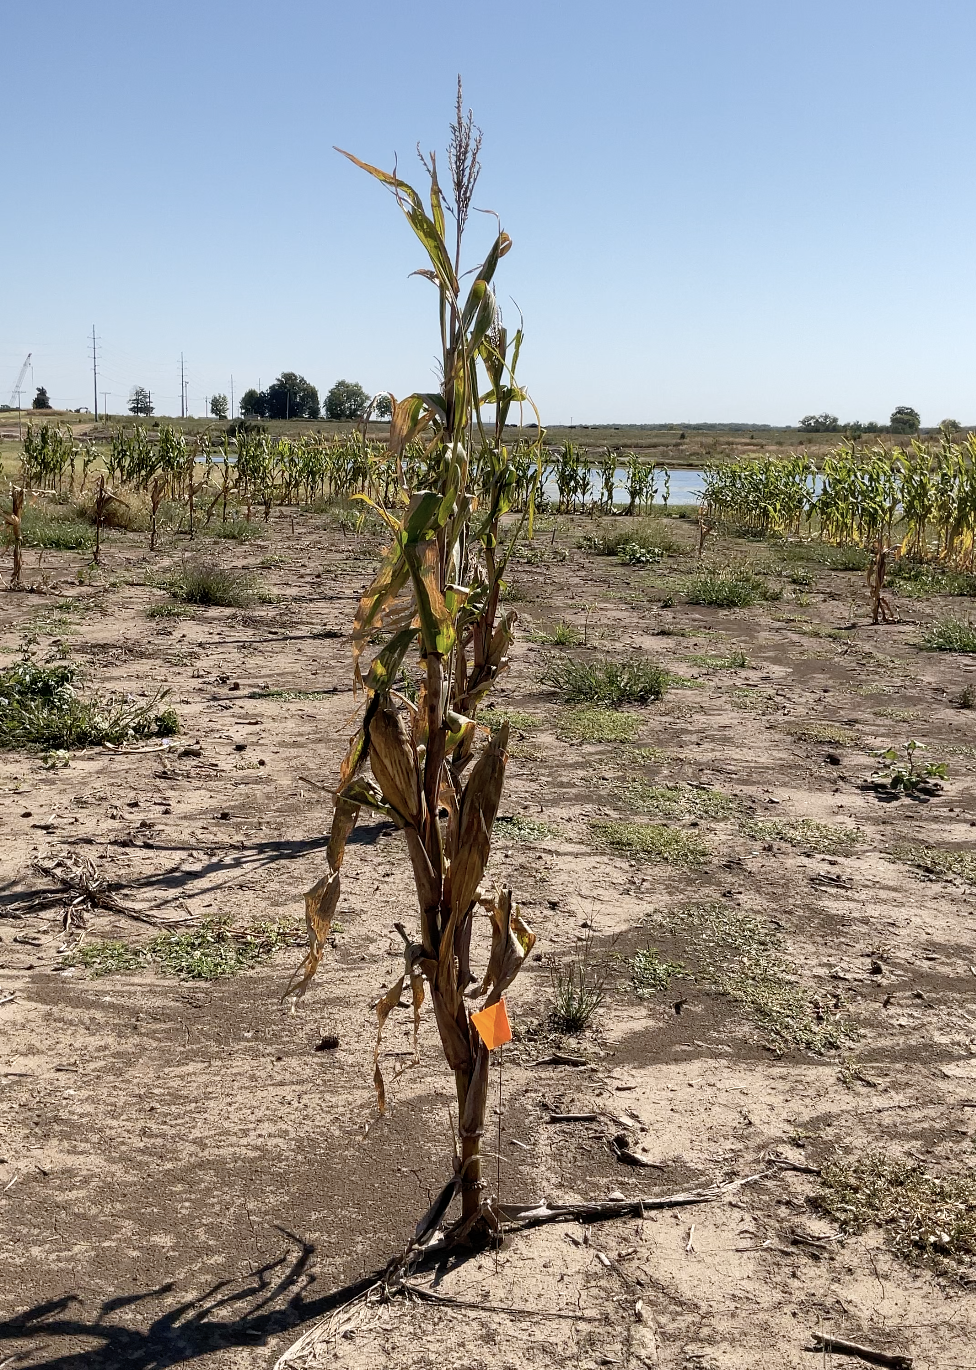
\includegraphics[align=c]{./images/meshlab/corn2_rgb.png}} &
\scalebox{0.125}{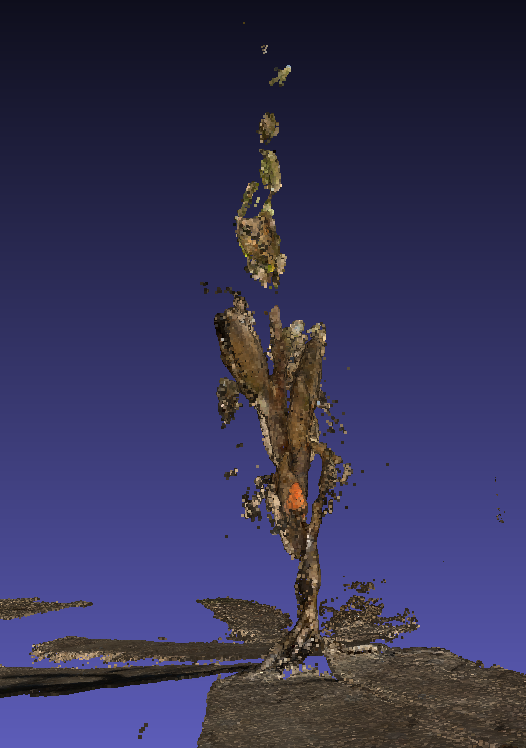
\includegraphics[align=c]{./images/meshlab/corn2_3dScanner_pc.png}} &
\scalebox{0.16}{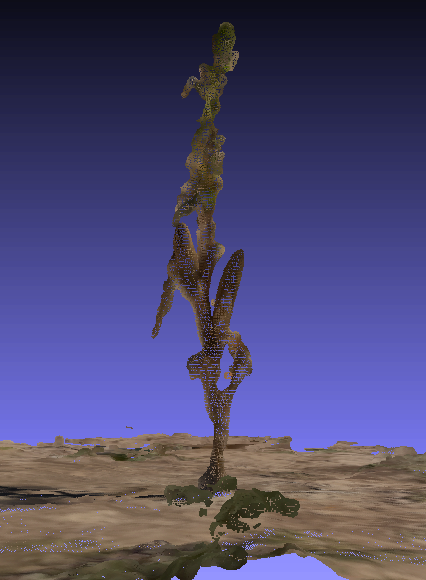
\includegraphics[align=c]{./images/meshlab/corn2_scaniverse_pc.png}}\\
%
\end{tabular}
}
\end{frame}



\begin{frame}[label={sec:org27d1adf}]{More Points make Smoother Plants}

\begin{center}
\begin{tabular}{l|rr}
plant & \tdsapp & Scaniverse\\
\hline
soybean & 197,819 & 1,289,299\\
cocklebur & 53,913 & 1,102,817\\
maize & 96,807 & 1,503,680\\
\end{tabular}
\end{center}
\end{frame}



\begin{frame}[label={sec:org8354af7}]{Thanks!}
\begin{itemize}
\item The organizers

\item Missouri Maize Center and especially Chris Browne
\item Dept. of Electrical Engineering and Computer Science Graduate
Fellowship
\item an anonymous gift

\item and you!

\end{itemize}
\end{frame}
\end{document}
